%%%%%%%%%%%%%%%%%%%%%%%%%%%%%%%%%%%%%%%%%%%%%%%%%%%%%%%%%%%%
\documentclass[xcolor=x11names,compress]{beamer}

\definecolor{CoolBlack}{rgb}{0.0, 0.18, 0.39}
\definecolor{byellow}{rgb}{0.55037, 0.38821, 0.06142}
%% General document %%%%%%%%%%%%%%%%%%%%%%%%%%%%%%%%%%
\usepackage{graphicx}
\usepackage{tikz}
\usepackage{Tabbing}
\usetikzlibrary{decorations.fractals}
%%%%%%%%%%%%%%%%%%%%%%%%%%%%%%%%%%%%%%%%%%%%%%%%%%%%%%

%% Beamer Layout %%%%%%%%%%%%%%%%%%%%%%%%%%%%%%%%%%
\useoutertheme[subsection=false,shadow]{miniframes}
\useinnertheme{default}
\usefonttheme{serif}
\usepackage{palatino}
\usepackage{tabu}

% addition of color
\usepackage{xcolor}
\definecolor{dgreen}{rgb}{0.,0.6,0.}
\definecolor{RawSienna}{cmyk}{0,0.72,1,0.45}

\setbeamerfont{title like}{shape=\scshape}
\setbeamerfont{frametitle}{shape=\scshape}

\setbeamercolor*{lower separation line head}{bg=CoolBlack} 
\setbeamercolor*{normal text}{fg=black,bg=white} 
\setbeamercolor*{alerted text}{fg=red} 
\setbeamercolor*{example text}{fg=black} 
\setbeamercolor*{structure}{fg=black} 
 
\setbeamercolor*{palette tertiary}{fg=black,bg=black!10} 
\setbeamercolor*{palette quaternary}{fg=black,bg=black!10} 

\renewcommand{\(}{\begin{columns}}
\renewcommand{\)}{\end{columns}}
\newcommand{\<}[1]{\begin{column}{#1}}
\renewcommand{\>}{\end{column}}

% adding slide numbers
\addtobeamertemplate{navigation symbols}{}{%
    \usebeamerfont{footline}%
    \usebeamercolor[fg]{footline}%
    \hspace{1em}%
    \insertframenumber/\inserttotalframenumber
}

% equation stuff
\newcommand{\Macro}{\ensuremath{\Sigma}}
\newcommand{\Sn}{\ensuremath{S_N} }
\newcommand{\vOmega}{\ensuremath{\hat{\Omega}}}
\usepackage{mathrsfs}
\usepackage[mathcal]{euscript}
\usepackage{amssymb}
\usepackage{amsthm}
\usepackage{epsfig}
\usepackage{amsmath}

\newcommand{\ve}[1]{\ensuremath{\mathbf{#1}}}
\newcommand{\micro}{\ensuremath{\sigma}}
\newcommand{\detR}{\ensuremath{\Sigma}}
%%%%%%%%%%%%%%%%%%%%%%%%%%%%%%%%%%%%%%%%%%%%%%%%%%

\begin{document}

%%%%%%%%%%%%%%%%%%%%%%%%%%%%%%%%%%%%%%%%%%%%%%%%%%%%%%
%%%%%%%%%%%%%%%%%%%%%%%%%%%%%%%%%%%%%%%%%%%%%%%%%%%%%%
\begin{frame}
\title{Recent Past and Planned Research}
\subtitle{Reactor Design and Neutronics Group}
\author{
        \includegraphics[height=2cm]{bk}\\R.\ N.\ Slaybaugh}

\date{April 15, 2014}
\titlepage
\end{frame}

% --------------------------------------------------------------
\begin{frame}[fragile]{Outline}
  \frametitle{Outline}
  \begin{itemize}
    \item Hybrid methods overview
    \begin{itemize}
     	\item Motivation
		\item CADIS
		\item FW-CADIS
		\item Challenges
    \end{itemize}
	\item MC importances in the presence of space and energy self-shielding
	\begin{itemize}
    		\item Cross Section Processing
		\item Problem Investigation
		\item Resonance Factor Method
		\item Results
		\item Summary and Conclusions
  	\end{itemize}
	\item MC importances for problems with strong anisotropies
	\item Other potential projects
  \end{itemize}

\end{frame}


% --------------------------------------------------------------
% --------------------------------------------------------------
\section{\scshape Hybrid Methods}
%\subsection{Motivation}
\begin{frame}[fragile]
  \frametitle{Solving the TE}

\begin{columns}
  \begin{column}{0.5\textwidth}
  \begin{center}
  \underline{Monte Carlo}
  \end{center}
	\begin{itemize}
	\item Solution has associated statistical error
	\item Continuous phase space: ``gold standard answers"
	\item Can take a long time
	\item Good for streaming
	\item Optically thick = slow
	\end{itemize}
  \end{column}
  \begin{column}{0.5\textwidth}
  \begin{center}
  \underline{Deterministic}
  \end{center}
	\begin{itemize}
	\item Solution equally valid everywhere
	\item Discretized phase space: drives solution quality
	\item Can be fast
	\item Streaming = ray effects
	\item Good for optically thick
	\end{itemize}
  \end{column}
\end{columns}

\end{frame}

% --------------------------------------------------------------
\begin{frame}[fragile]
  \frametitle{Acceleration}
  \begin{itemize}
  	\item To use MC in many applications, we need to \textit{accelerate} it
	\item Variance reduction is designed to improve the FOM:
  \end{itemize}
\begin{align}
\text{FOM} = \frac{1}{\text{R}^2\text{t}} \qquad & \text{R = relative error} \nonumber \\ 
& \text{t = time} \nonumber 
\end{align}
  \begin{itemize}
  	\item \underline{Idea}: can we use deterministic and Monte Carlo methods together to lessen the weaknesses of each?
  \end{itemize}
  $\rightarrow$ \textbf{Hybrid Methods}

\end{frame}


% --------------------------------------------------------------
%\subsection{CADIS}
\begin{frame}[fragile]
  \frametitle{CADIS}
Define response with function $f(\ve{r}, E)$ in volume, $V_d$ as
%
\begin{equation}
 R = \int_E \int_{V_f} f(\ve{r}, E) \phi(\ve{r}, E) dV dE 
 \label{eq:Response}
\end{equation}
%
\begin{columns}
  \begin{column}{0.5\textwidth}
	\begin{align}
  	H\phi &= q \quad \text{(forward)}\nonumber \\
  	%
  	H^{\dagger} \phi^{\dagger} &= q^{\dagger} \quad 
  	\text{(adjoint)}\nonumber
  	\end{align}
  \end{column}
  \begin{column}{0.5\textwidth}
  	\begin{align}
  	\langle H\phi, \phi^{\dagger} \rangle &= \langle H^{\dagger} \phi^{\dagger}, \phi \rangle \:, \text{and therefore} \nonumber \\
  	%
  	\langle q, \phi^{\dagger} \rangle &= \langle q^{\dagger}, \phi \rangle \nonumber
  	\end{align}
  \end{column}
\end{columns}
\vspace*{1 em}
If we let $q^{\dagger} = f(\ve{r}, E)$ then
%
\begin{equation}
 \langle q^{\dagger}, \phi \rangle = \langle f, \phi \rangle = R = \langle q, \phi^{\dagger} \rangle
 \label{eq:ResponseRedef}
\end{equation}
%
Eq.\ \eqref{eq:ResponseRedef} expresses that $\phi^{\dagger}$ represents the expected contribution of a source particle to the response given the source, $q$.

\end{frame}

% --------------------------------------------------------------
\begin{frame}[fragile]
  \frametitle{CADIS}
  
  \begin{enumerate}
  \item Define $q^{\dagger}$ as the local response of interest\\
  \item Generate $\phi^{\dagger}$ and $R$ with a coarse deterministic solution
  \end{enumerate}
% 
\begin{align}
  imp(\ve{r}, E) &= \frac{\phi^{\dagger}(\ve{r}, E)}{\langle q(\ve{r}, E), \phi^{\dagger}(\ve{r}, E) \rangle} = \frac{\phi^{\dagger}(\ve{r}, E)}{R(\ve{r}, E)} \\
  %
  \hat{q}(\ve{r}, E) &= \frac{\phi^{\dagger}(\ve{r}, E) q(\ve{r}, E)}{R} \\
  %
  w_0(\ve{r}, E) &= \frac{q(\ve{r}, E)}{\hat{q}(\ve{r}, E)} = \frac{R}{\phi^{\dagger}(\ve{r}, E)} 
  \label{eq:Importance}
\end{align}

Birth weights match weight targets, making this the \underline{C}onsistent \underline{A}djoint \underline{D}riven \underline{I}mportance \underline{S}ampling \underline{M}ethod

\end{frame}

% --------------------------------------------------------------
%\subsection{FW-CADIS}
\begin{frame}[fragile]
  \frametitle{FW-CADIS}

\begin{itemize}
\item We often what to optimize solutions in all of phase space\\
\item In this case the adjoint source needs to be a global forward solution: \underline{F}orward \underline{W}eighted-CADIS
\end{itemize}
%
\begin{columns}
  \begin{column}{0.5\textwidth}
  \begin{center}
  \textcolor{byellow}{To Optimize}
  \end{center}
	\begin{align}
  	&\phi(\ve{r}, E)\nonumber \\
  	%
  	\int&\phi(\ve{r}, E)\sigma_d(\ve{r}, E)\nonumber
  	\end{align}
  \end{column}
  %
  \begin{column}{0.5\textwidth}
  \begin{center}
  \textcolor{byellow}{Adjoint Source}
  \end{center}
  	\begin{align}
  	f(\ve{r}, E) &= \frac{1}{\phi(\ve{r}, E)}\nonumber \\
  	%
  	f(\ve{r}, E) &= \frac{\sigma_d(\ve{r}, E)}{\int\phi(\ve{r}, E)\sigma_d(\ve{r}, E)} \nonumber
  	\end{align}
  \end{column}
\end{columns}
\vspace*{1 em}
For example
%
\begin{equation}
 R = \int_E \int_{V_f} f(\ve{r}, E) \phi(\ve{r}, E) dV dE = \int_E \int_{V} \frac{1}{\phi(\ve{r}, E)} \phi(\ve{r}, E) dV dE \approx 1 \nonumber
\end{equation}

\end{frame}

% --------------------------------------------------------------
%\subsection{Challenges}
\begin{frame}[fragile]
  \frametitle{Challenges}

	FW-CADIS works well for \textbf{most} deep penetration
	shielding problems...
	%
	\begin{columns}
  	\begin{column}{0.5\textwidth}
  	\begin{figure}
  	\begin{center}
  		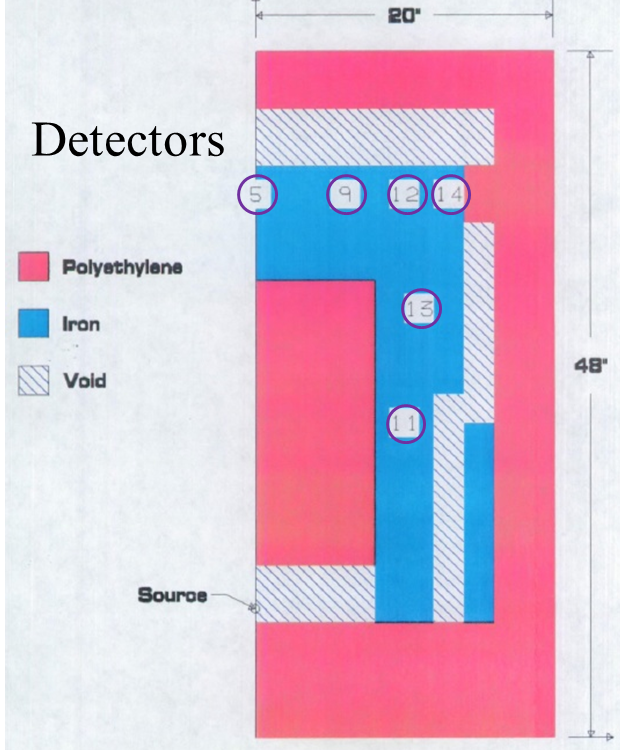
\includegraphics[height=2in,clip]{dlvn}
		\caption{Dog Legged Void Neutron Shielding Benchmark}
	\end{center}
  	\end{figure}
  	\end{column}
 	%
 	\begin{column}{0.5\textwidth}
 	\begin{figure}
  	\begin{center}
  		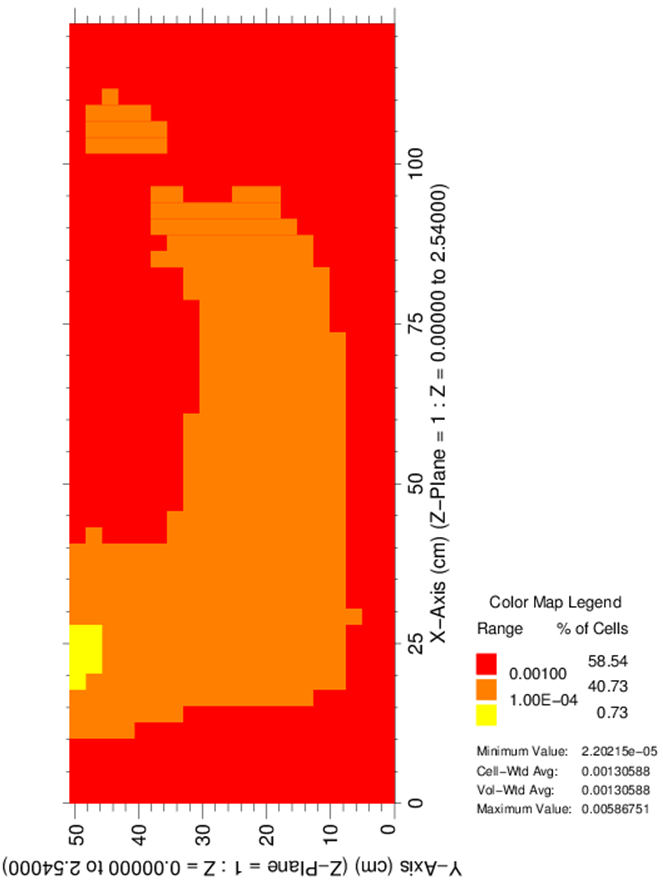
\includegraphics[height=2in,clip]{dlvn-lowVR}
  		\caption{MC 95\% CI RE using FW-CADIS, DLVN}
  	\end{center}
  	\end{figure}
  	\end{column}
	\end{columns}
  
\end{frame}

% --------------------------------------------------------------
\begin{frame}[fragile]
  \frametitle{Challenges}

	...but not all of them
	%
	\begin{columns}
  	\begin{column}{0.5\textwidth}
  	\begin{center}
		\begin{itemize}
		\item FW-CADIS only includes space and energy, 
			\textit{not angle}
		\item One pathological case:
		\begin{itemize}
		\item Energy self-shielding +
		\item Spatial self-shielding
		\end{itemize}
		\item High relative error through location of Interest
		\item Outcome: new methods based on FW-CADIS
		\item The Resonance Factor method uses different cross section processing
		\end{itemize}
	\end{center}
  	\end{column}
 	%
 	\begin{column}{0.5\textwidth}
  	\begin{center}
  	\begin{figure}
  		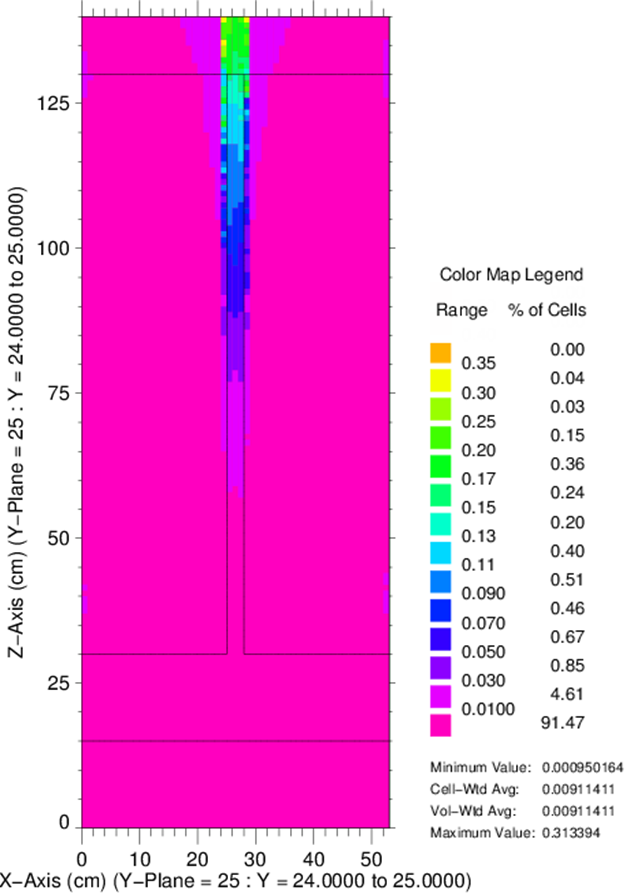
\includegraphics[height=2in,clip]{plate-badVR}
  		\caption{MC 95\% CI RE using FW-CADIS, Plate}
  	\end{figure}
  	\end{center}
  	\end{column}
	\end{columns}
  
\end{frame}


% --------------------------------------------------------------
% --------------------------------------------------------------
\section{Self-Shielding}
%\subsection{Cross Section Processing}
\begin{frame}[fragile]
  \frametitle{Cross Section Processing}

	\begin{itemize}
	\item General Case
	\begin{equation}
  	\micro_{x,g}^{(j)} = \frac{\langle \micro_x^{(j)}(u) W(u)\rangle}
	{\langle W(u)\rangle} \:, \quad W(u) = \phi_{\infty}(u)
 	 \label{eq:baseBondarenko}
 	\end{equation} 
 	
 	\item Bondarekno method uses a background cross section
 	\begin{equation}
  	\micro_0^{(j)} = \frac{1}{N_j} \sum_{m \ne j} \micro_{t}^{(m)} N_m 
  	%\label{eq:bgxsec}
  	\:, \quad \micro_{x,g}^{(j)}(\micro_0^{(j)}y) = \frac{\langle
  	 \micro_{x}^{(j)}(u) \frac{\phi_{\infty}(u)} {\micro_{t}^{(j)}(u)
  	 + \micro_0^{(j)}} \rangle}
  	 { \langle \frac{\phi_{\infty}(u)}{\micro_{t}^{(j)}(u) +
  	 \micro_0^{(j)}}\rangle}
  \label{eq:ssfact}
	\end{equation}

	\item W(u) changed to include the  spectral difference assumption and effect of other isotopes
	\end{itemize}
	
\end{frame}
	
% --------------------------------------------------------------
\begin{frame}[fragile]
  \frametitle{Cross Section Processing}

	\begin{itemize}
	\item When When a nuclide is dilute, $\sigma_0^{(j)} >>
	 \sigma_t^{(j)}$, \\$W(u) \rightarrow$ uncorrected 
		\begin{itemize}
		\item Large $\sigma_0$ = infinitely dilute case	
		\end{itemize}

	\item When a nuclide is concentrated, $\sigma_0^{(j)} << 
	 \sigma_t^{(j)}$, resonances have a larger impact 
		\begin{itemize}
		\item Small $\sigma_0$ = resonance case	
		\end{itemize}
	\end{itemize}
	
	\begin{itemize}
	\item Add correction for `thin slab' of resonance material in 
	`thick slab' of moderator
	\begin{align}
  	&\sigma_0^{*,(j)} = \frac{1}{N_j} \sum_{m \ne j} \sigma_{t}^{(m)} N_m 
	+ \frac{1}{N_j \bar{l}} \\
  	&\text{\textcolor{byellow}{thin slab:}}\:\bar{l} \approx \frac{4V}{S} \qquad \text{\textcolor{byellow}{no effect:}}\:\bar{l} \approx \text{large} \nonumber
	\end{align}
	\end{itemize}
  
\end{frame}

% --------------------------------------------------------------
%\subsection{Problem Investigation}
\begin{frame}[fragile]
  \frametitle{Problem Investigation}
  	\begin{columns}
  	\begin{column}{0.45\textwidth}
  	\begin{figure}
  		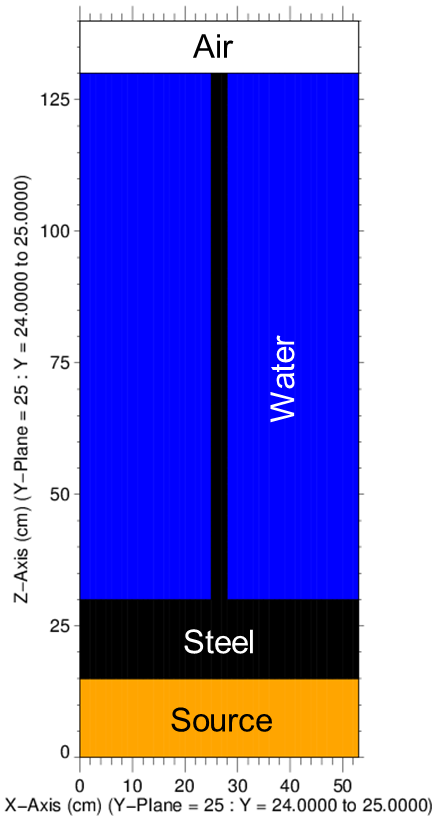
\includegraphics[height=2in,clip]{plate-geometry}
  		\caption{Shielding Stack Up}
  	\end{figure}
  	\end{column}
 	%
 	\begin{column}{0.6\textwidth}
	\begin{itemize}
	\item 53 cm $\times$ 50 cm $\times$ 140 cm 
	\item Uniform in x except plate (25-28 cm in x; 30-130 cm in z)
	\item Uniform in y
	\item U-235 fission spectrum; homogenized U, Zr, and H2O
	\vspace*{1 em}
	\item MC21, MCNP, and PARTISN
	\item ENDF/B-VII data (all codes)
	\item Processed by TRANSX (multigroup)
	\end{itemize}
  	\end{column}
	\end{columns}
  
\end{frame}


% --------------------------------------------------------------
\begin{frame}[fragile]
  \frametitle{Base Calculation Parameters}
  \begin{table}[p]
  \label{tab:calcParams}
  \begin{center}
    \begin{tabu}{| X | X | X |}\hline
      Variable & PARTISN & MC21\\\hline\hline
	Deterministic Mesh & 0.5 cm unif; 0.25 cm in $x$ over 24 to 29 cm & 1 cm uniform \\\hline
	Tally mesh & N/A & 1 cm uniform \\\hline
	N particles & N/A & $1 \times 10^{10}$\\\hline
	Energy structure & 58 grps & 27 grps / continuous\\\hline
	Angular quad & QR-18-252 & QR-8-36\\\hline
	Scattering order & $P_3$ & $P_3$\\\hline
	Convergence & 0.01 & 0.05\\\hline
	TRANSX settings & default & default\\\hline
	DCFs & 58 grps & 27 grps \\\hline
    \end{tabu}
  \end{center}
\end{table}
  
\end{frame}

% --------------------------------------------------------------
\begin{frame}[fragile]
  \frametitle{Errors in Plate}
 \begin{figure}[p]
   \begin{center}
     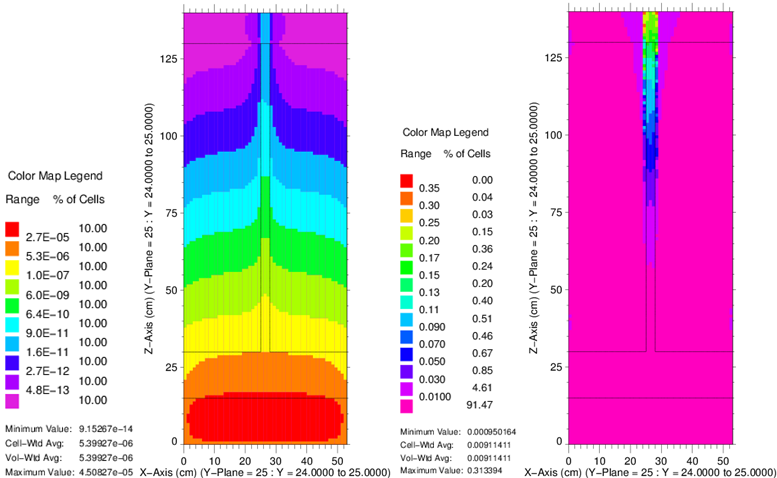
\includegraphics[height=2 in,clip]{NSE13-109R1-PlateDRandRE}
   \end{center}
   \caption{Plate base FW-CADIS MC21 dose rate (left) and 95CI RE (right) (xz-slice through y=25 cm)}
   \label{fig:Plate}
 \end{figure}
\end{frame}

% --------------------------------------------------------------
\begin{frame}[fragile]
  \frametitle{Correct Without Plate}
 \begin{figure}[p]
   \begin{center}
     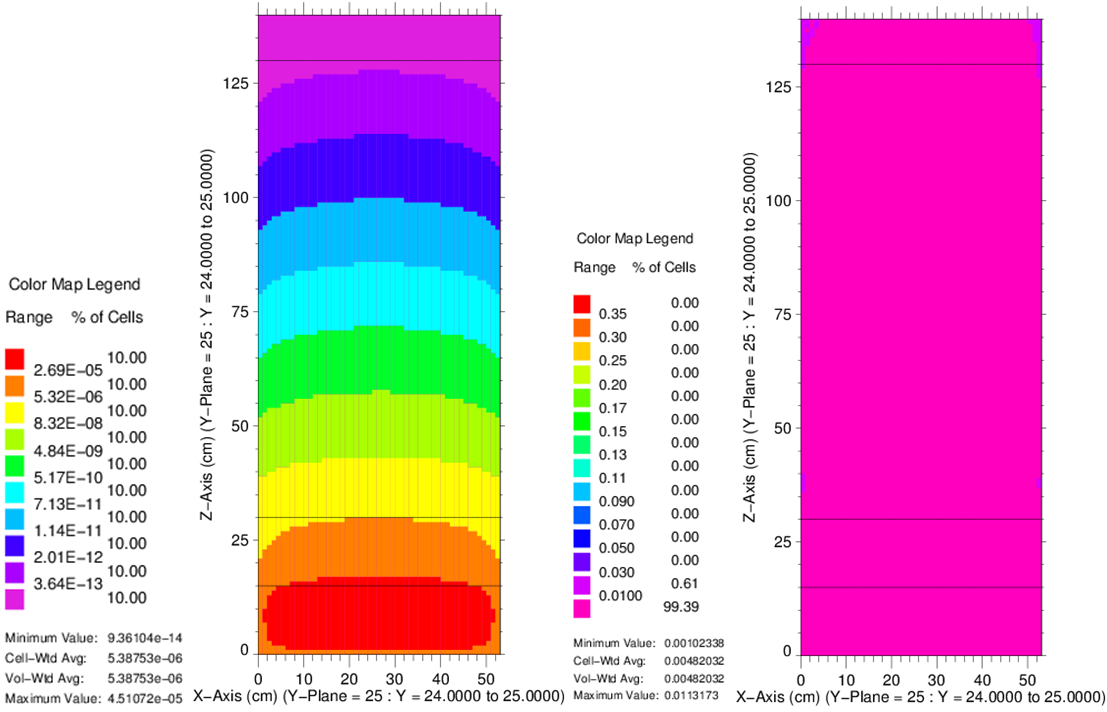
\includegraphics[height=2in,clip]{NSE13-109R1-NoPlateDRandRE}
   \end{center}
   \caption{No-Plate MC21 dose rate (left) and 95CI RE (right) (xz-slice through y=25 cm)}
   \label{fig:noPlate}
 \end{figure}
\end{frame}

% --------------------------------------------------------------
\begin{frame}[fragile]
  \frametitle{Deterministic MC Mismatch}
 \begin{figure}[p]
   \begin{center}
     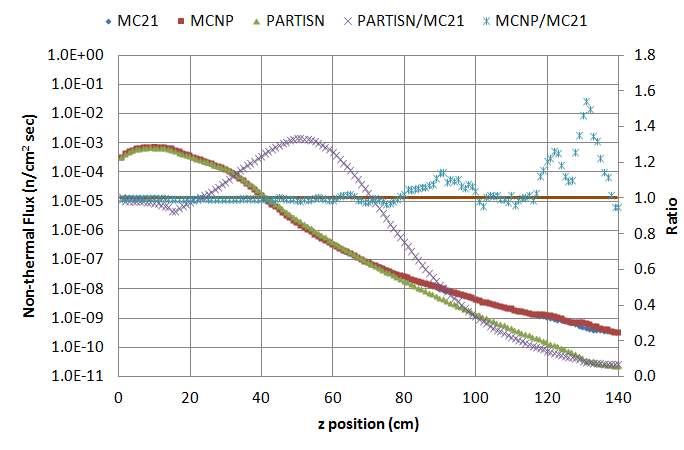
\includegraphics[width=4in,clip]{NSE13-109R1-PlateFluxExcel}
   \end{center}
   \caption{Plate non-thermal flux (left axis) and method ratios (right axis) down the x-y centerline}
   \label{fig:PlateFlux}
 \end{figure}
\end{frame}

% --------------------------------------------------------------
\begin{frame}[fragile]
  \frametitle{Deterministic MC Mismatch}
 \begin{figure}[p]
   \begin{center}
     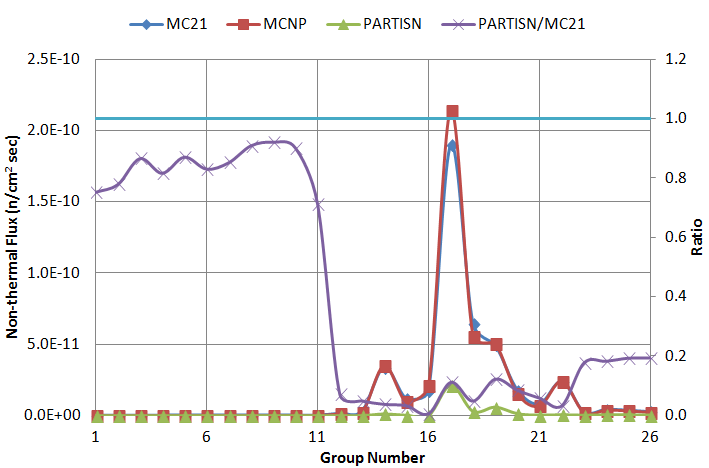
\includegraphics[width=4in,clip]{NSE13-109R1-PlateExitSpectra}
   \end{center}
   \caption{Plate flux spectra (left axis) and PARTSN/MC21 (right axis) at start of air region (z = 130.5 cm)}
   \label{fig:PlateExit}
 \end{figure}
\end{frame}

% --------------------------------------------------------------
\begin{frame}[fragile]
  \frametitle{Correct Without Plate}
 \begin{figure}[p]
   \begin{center}
     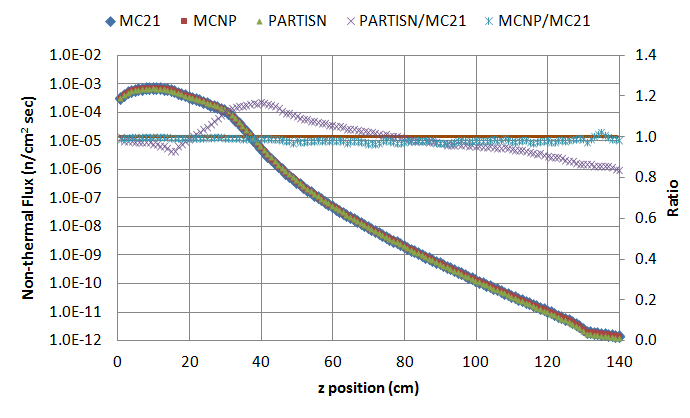
\includegraphics[width=4in,clip]{NSE13-109R1-NoPlateFluxExcel}
   \end{center}
   \caption{Plate non-thermal flux (left axis) and method ratios (right axis) down the x-y centerline}
   \label{fig:noPlateFlux}
 \end{figure}
\end{frame}

% --------------------------------------------------------------
\begin{frame}[fragile]
  \frametitle{Investigation}

	\begin{itemize}
	\item Parameters
	\begin{tabbing}
	* Mean chord length: \hspace*{1em} \= $\bar{l} = \frac{4V}{S}$ vs.\ $\bar{l} = 10,000$ \\
	* Angular quadrature: \> CMG-591 vs.\ QR-18-252 \\
	* Scattering expansion: \> P$_{5}$ vs.\ P$_{3}$ \\
	* Importance mesh: 	\> 0.25 cm (x), 0.5 cm (y,z) \\ \> in plate vs. 1 cm \\
	* Energy Structure: 	\> 58 vs.\ 27 groups
	\end{tabbing}
	
	\item CADIS in 2 cm area following plate
	\end{itemize}
	%
	\begin{columns}
  	\begin{column}{0.65\textwidth}
	\begin{itemize}
	\item Physics
		\begin{itemize}
		\item Polyethylene follow-on
		\item Cr plate (different resonance material)
		\item Air in plate (no resonance material)
		\end{itemize}
	\end{itemize}
  	\end{column}
  	%
 	\begin{column}{0.35\textwidth}
 	\begin{align}
 	\text{FOM}_{\min} &= \frac{1}{Rt_{\max}^2} \nonumber \\
 	\text{FOM}_{\max} &= \frac{1}{Rt_{\min}^2} \nonumber
 	\end{align}
 	\end{column}
	\end{columns}
  
\end{frame}

% --------------------------------------------------------------
\begin{frame}[fragile]
  \frametitle{Parameters Results}
  
  	\begin{itemize}
  	\item Geometric chord length $\rightarrow$ PARTISN flux even farther from correct, especially in plate
  	\item Angular quadrature $\rightarrow$ no differences with impact
	\item Scattering order $\rightarrow$ (nearly) no change
  	\end{itemize}
  	
  \begin{center}
    \begin{tabu}{|l|r|r|r|r|r|r|}\hline
      Case & NPS & CPU-hrs & Max RE & Avg RE & Min F & Avg F\\\hline
      %%
Base      & 1e10 & 849.77    & 8.10e-1 & 1.02e-2 & 1.79e-3 & 11.3\\
%
1e11 & 1e11 & 8,543.47  & 1.64e-1 & 3.28e-3 & 4.33e-3 & 10.9\\
%
58 g & 1e10 & 954.89    & 5.22e-1 & 9.33e-3 & 3.85e-3 & 12.0\\
%
Fine & 1e10 & 905.34    & 1.55  & 1.71e-2 & 4.63e-4 & 3.78\\
%
F2e11 & 2e11 & 18,367.67 & 3.43e-1 & 4.00e-3 & 4.62e-4 & 3.40\\\hline
    \end{tabu}
  \end{center}

\end{frame}

% --------------------------------------------------------------
\begin{frame}[fragile]
  \frametitle{CADIS, Poly Follow}
 \begin{figure}[p]
   \begin{center}
     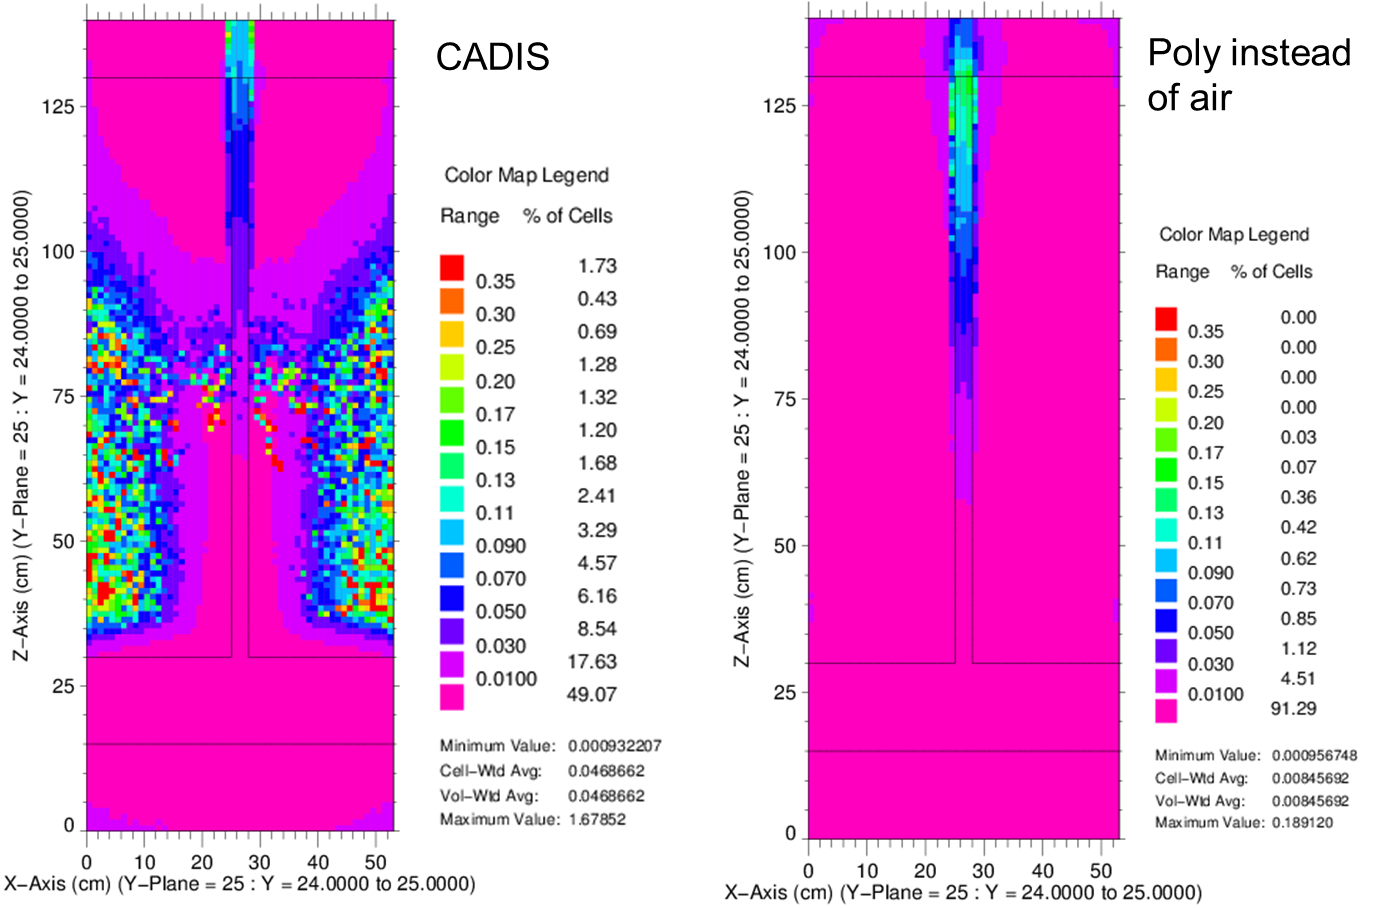
\includegraphics[width=4in,clip]{cadis-poly}
   \end{center}
 \end{figure}
\end{frame}

% --------------------------------------------------------------
\begin{frame}[fragile]
  \frametitle{Resonance Streaming}
   \begin{figure}[p]
   \begin{center}
     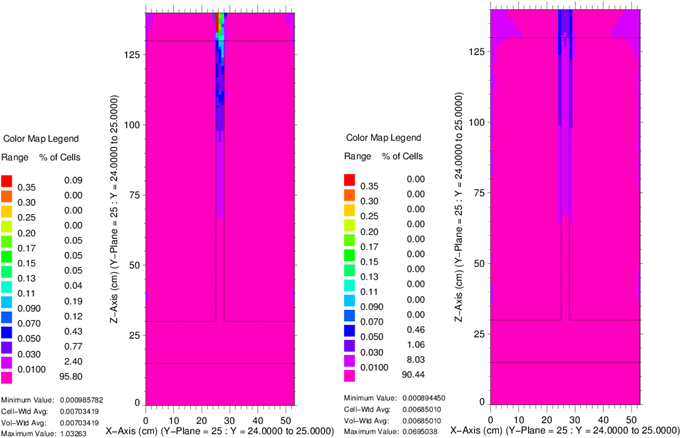
\includegraphics[width=4in,clip]{NSE13-109R1-CrAir}
   \end{center}
   \caption{Cr plate (left) and air plate (right) FW-CADIS MC21 dose rate 95CI RE (xz-slice through y=25 cm)}
   \label{fig:CrAir}
 \end{figure}
\end{frame}

% --------------------------------------------------------------
\begin{frame}[fragile]
  \frametitle{MAVRIC}
  
  \begin{itemize}
  \item We also ran this problem with and without the plate in MAVRIC (a multigroup MC code in SCALE)
  \item MAVRIC has more advanced cross section processing options
  \item Used 27 g and 200 g
  \item One 200 g case the plate was broken into 9 separate 10-cm segments – each with different xsecs
  \item Without plate case was correct
  \item 27 g $\rightarrow$ completely missed the behavior
  \item Both 200 g cases $\rightarrow$ exhibited the same streaming and high relative error behavior
  \end{itemize}
  
\end{frame}

% --------------------------------------------------------------
\begin{frame}[fragile]
  \frametitle{Investigation Summary}
  
	\begin{itemize}
	\item Behavior is related to space and energy self-shielding
	
	\item Using these items did not improve PARTISN
	 \begin{itemize}
	 \item finer quadrature
	 \item higher scattering order
	 \item more theoretically-accurate mean chord length
	 \end{itemize}
	 
	\item Using these items in imp map creation did not reduce REs
	 \begin{itemize}
	 \item finer spatial mesh in the problem area
	 \item finer energy group structure to create the importance map
	 \end{itemize}
	 
	\item The high RE in and following the plate is present when using different codes and different methods to produce VR parameters, and exists when a different resonance material is used.
	\end{itemize}


A sufficiently accurate PARTISN solution would be better (probably), but prohibitively expensive.
  
\end{frame}


% --------------------------------------------------------------
% --------------------------------------------------------------
%\subsection{Resonance Factor Method}
\begin{frame}[fragile]
  \frametitle{Resonance Factor Method}
  	Apply renormalization factor to FW-CADIS source $q^{\dagger}_{FWC}$: 
	%
	\begin{equation}
   	q^{\dagger}(\ve{r},E) = \Bigl(\frac{\phi_{res(\micro_0)}(\ve{r},E)}{\phi_{dilute(\micro_0)}(\ve{r},E)}\Bigr)^M q^{\dagger}_{FWC} 
  	 \label{eq:newQ}
	\end{equation}
	%
	where
	\begin{itemize}
  	\item M is problem-dependent constant 
 	 \item $\phi_{res(\micro_0)}(\ve{r},E)$ is forward flux using a small background xsec
 	 \item $\phi_{dilute(\micro_0)}(\ve{r},E)$ is forward flux using a large background xsec
	\end{itemize}
	
	The resulting adjoint flux is used to make importances
	\vspace*{1 em}
	
	Implementation: use $\phi_{res(\micro_0)}(\ve{r},E)$  in all locations where $\phi$ would be used in the FW-CADIS method
	
	
	
\end{frame}

% --------------------------------------------------------------
\begin{frame}[fragile]
  \frametitle{Resonance Factor Method}
  
	Example: optimize the space- and energy-dependent flux
	
	\vspace*{1 em}
	$q^{\dagger}_{FWC} = 1 / \phi$ and results in this corrected response: 
	%
	\begin{align}
 	R &= \int_E \int_{V} \Bigl(\frac{\phi_{res(\micro_0)}(\ve{r},E)}{\phi_{dilute(\micro_0)}(\ve{r},E)}\Bigr)^M \frac{1}{\phi_{res(\micro_0)}(\ve{r}, E)} \phi_{res(\micro_0)}(\ve{r}, E) dV dE \nonumber
 	\label{eq:newResponse} \\
  	 &\approx \int_E \int_{V} \Bigl(\frac{\phi_{res(\micro_0)}(\ve{r},E)}{\phi_{dilute(\micro_0)}(\ve{r},E)}\Bigr)^M dV dE \:. \nonumber
	\end{align}
	%
	The expanded version of importance map in plate becomes:
	%
	\begin{equation}
 imp(\ve{r},E)= \frac{\phi_{res(\micro_0)}^{\dagger}(\ve{r},E)}{\int_E \int_{V} \bigl(\frac{\phi_{res(\micro_0)}(\ve{r},E)}{\phi_{dilute(\micro_0)}(\ve{r},E)}\bigr)^M dV dE}
 	 \label{eq:newImp}
	\end{equation}  
  
\end{frame}



% --------------------------------------------------------------
%\subsection{Results}
\begin{frame}[fragile]
  \frametitle{Results}
    \begin{center}
  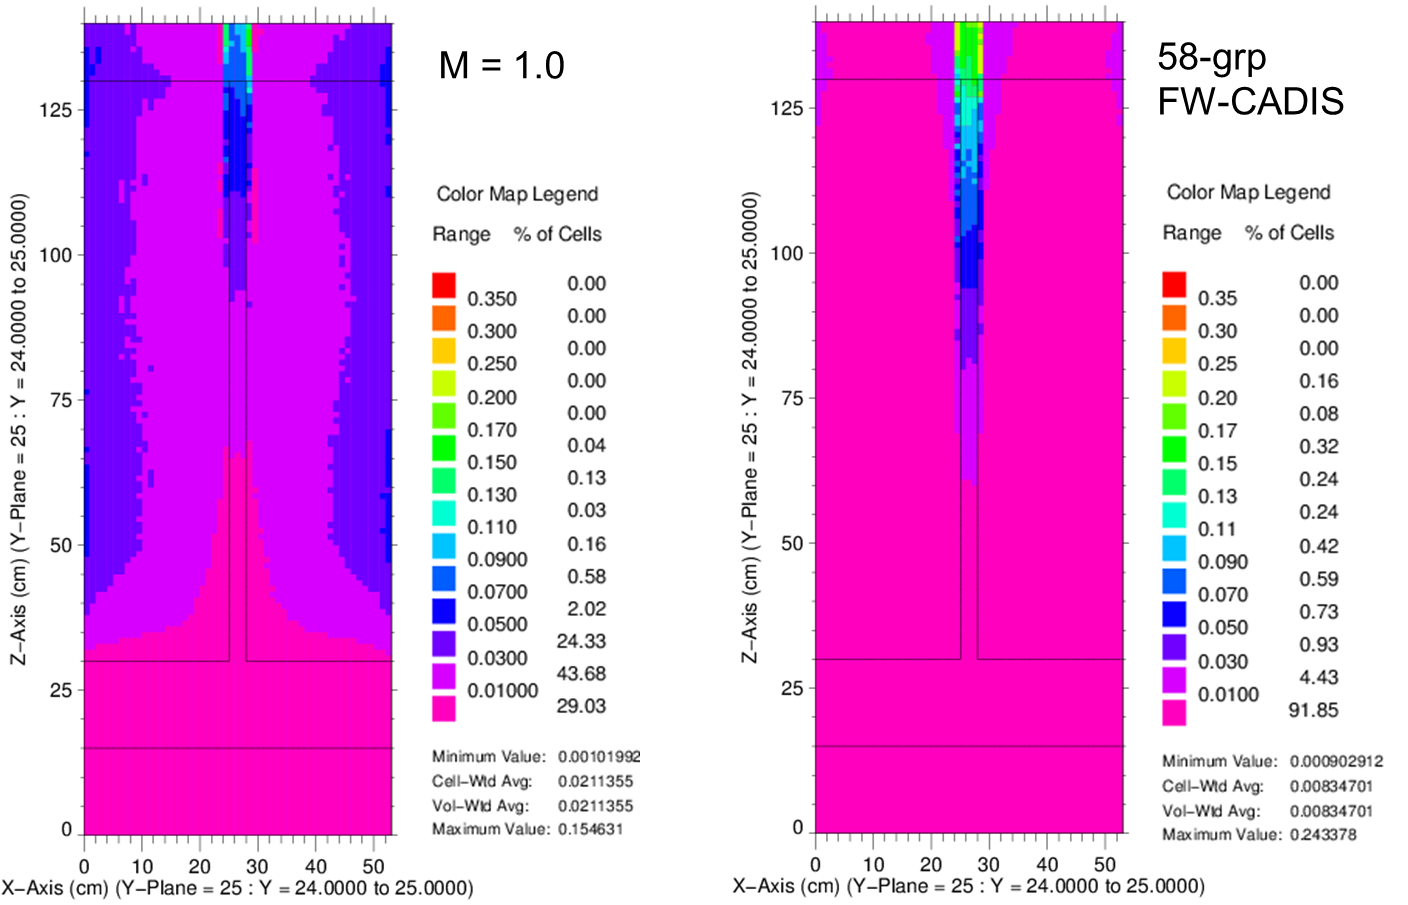
\includegraphics[width=4in,clip]{m1-vs-58g}  
  \end{center}
\end{frame}

% --------------------------------------------------------------
\begin{frame}[fragile]
  \frametitle{Results}

	\begin{table}[p]
 	 \label{tab:comparison}
  	\begin{center}
    \begin{tabular}{|l|r|r|r|r|r|}\hline
      Case & CPU-hrs & Max RE & Avg RE & Min FOM & Avg FOM\\\hline
      %%
base & 849.77 & 8.10e-1 & 1.02e-2 & 1.79e-3 & 11.3\\
%
58 g & 954.89 & 5.22e-1 & 9.33e-3 & 3.85e-3 & 12.0\\
%
M = 1 & 534.80 & 2.69e-1 & 2.44e-2 & 2.58e-2 & 3.13\\\hline
    \end{tabular}
 	 \end{center}
	\end{table}

	\begin{itemize}
	\item M = 1.0 used the same deterministic parameters as the base case
	\item FOM$_{\min}$ $\sim$10x better than best FW-CADIS case
	\item FOM$_{\min}$ and FOM$_{\text{avg}}$ are $\sim$100x closer together than best FW-CADIS case
	\end{itemize}

\end{frame}
%
%% --------------------------------------------------------------
%\begin{frame}[fragile]
%  \frametitle{Results}
%
%\end{frame}


% --------------------------------------------------------------
%\subsection{Summary and Conclusions}
\begin{frame}[fragile]
  \frametitle{Summary and Conclusions}
  
  \begin{itemize}
  \item Space and energy self-shielding make variance reduction difficult
  
  \item Caused by multigroup cross sections in angle-independent implementation
  
  \item Not resolved by
   \begin{itemize}
   \item Finer spatial mesh, energy group structure, or angular quadrature; higher order scattering expansion; or Bondarenko method
   \end{itemize}
   
  \item New method
   \begin{itemize}
  	\item Adds a factor accounting for resonances to FW-CADIS adjoint source
  	\item Tunable based on degree of problem manifestation
	\item Lowers FOM$_{\min}$ and brings FOM$_{\min}$ closer to FOM$_{\text{avg}}$
	\item More work, but useful in these pathological cases
   \end{itemize}
  \end{itemize}

\end{frame}


% --------------------------------------------------------------
% --------------------------------------------------------------
\section{Strong Anisotropies}
\begin{frame}[fragile]
  \frametitle{Anisotropy: a computational challenge}

	\begin{columns}
  	\begin{column}{0.5\textwidth}
	\begin{itemize}
	\item Many important nuclear applications have strong anisotropies
	 \begin{itemize}
	 \item Used fuel casks
	 \item Reprocessing facilities
	 \item Reactor facilities
	 \item Active interrogation 
	 \end{itemize}
	\item These are difficult to capture with current tools:
	 \begin{itemize}
	 \item Ray effects with deterministic
	 \item Too slow with analog MC
	 \item Insufficient acceleration of MC with hybrid
	 \end{itemize}
	\end{itemize}
  	\end{column}
 	%
 	\begin{column}{0.5\textwidth}
 	 \begin{center}
 	 \begin{figure}
 	 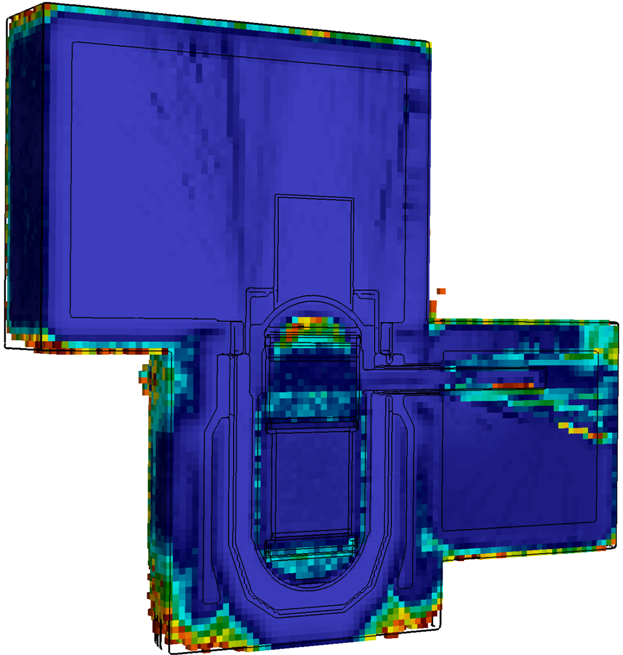
\includegraphics[height=2in,clip]{pwr}  
 	 \caption{PWR, 1 CPU-month, FW-CADIS  for mesh-tally (500K cells)}
 	 \end{figure}
 	 \end{center}

  	\end{column}
	\end{columns}

\end{frame}


% --------------------------------------------------------------
\begin{frame}[fragile]
  \frametitle{Current hybrid methods are insufficient}

	\begin{itemize}
	\item MC VR parameters created from adjoint deterministic flux that is a function of space and energy only
	\item Angular dependence of the importance function is not retained, otherwise the map would be very large (tens or hundreds of GB) and more costly and complex to use in the Monte Carlo simulation
	\item Drawback: within a given space/energy cell, the map provides the average importance of a particle moving in any direction through the cell—excluding information about how particles move toward the objective
	\end{itemize}

\end{frame}

% --------------------------------------------------------------
\begin{frame}[fragile]
  \frametitle{Current hybrid methods are insufficient}

	\begin{columns}
  	\begin{column}{0.5\textwidth}
 	 \begin{center}
 	 \begin{figure}
 	 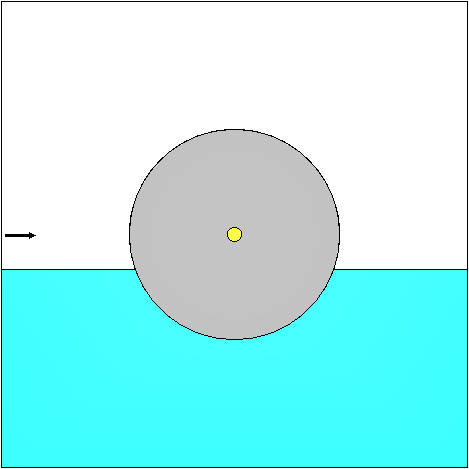
\includegraphics[height=2in,clip]{boat-interrogation}  
 	 \caption{Spherical boat model with source on left and fissionable material at center}
 	 \end{figure}
 	 \end{center}
  	\end{column}
 	%
 	\begin{column}{0.5\textwidth}
 	 \begin{center}
 	 \begin{figure}
 	 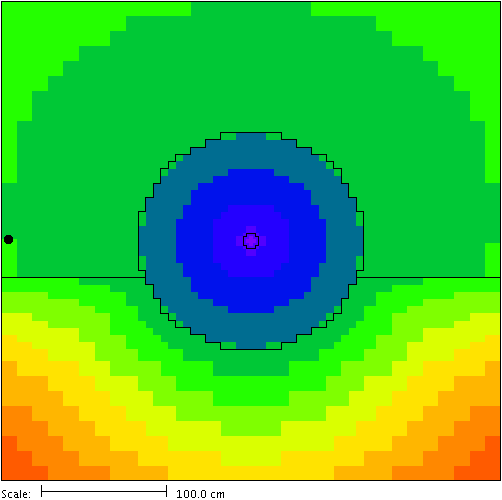
\includegraphics[height=2in,clip]{boat-map}  
 	 \caption{Target weight window values for 14.1 MeV neutrons}
 	 \end{figure}
 	 \end{center}
  	\end{column}
	\end{columns}

\end{frame}

% --------------------------------------------------------------
\begin{frame}[fragile]
  \frametitle{Better hybrid methods are needed}

	\begin{itemize}
	\item We can use angular information to improve performance
		\begin{equation}
		\phi^{\dagger}(\ve{r},E) = \frac{\int \psi(\vOmega, \ve{r},E) \psi^{\dagger}(\vOmega, \ve{r},E) d\vOmega}{\int \psi(\vOmega, \ve{r},E)  d\vOmega}
		\end{equation}

	\item The space- and energy-dependent importance map will be normalized and source biasing parameters will be generated in a manner similar to the current implementation of hybrid methods
	\item Immediately useful; widely applicable
	\end{itemize}

\end{frame}



% --------------------------------------------------------------
% --------------------------------------------------------------
\section{Other Projects}
\begin{frame}[fragile]
  \frametitle{Other (potential) projects}

  	\begin{itemize}
  	\item Continuing development of MC on GPU
	\item 3D shielding optimization: applicable to SMRs
	\item Parallelization of open source deterministic code 
	\item Hartouni Method
	\item Using SP$_N$ in multigrid preconditioner in Denovo
	\end{itemize}
	
\end{frame}


% --------------------------------------------------------------
% --------------------------------------------------------------
\section*{}
\begin{frame}[fragile]
  \frametitle{Questions?}
  \begin{center}
  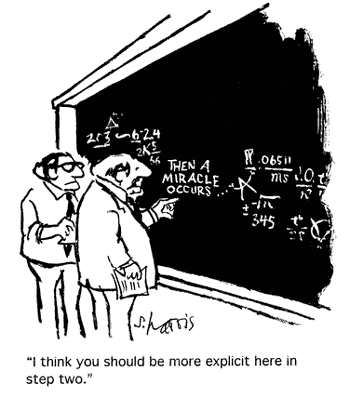
\includegraphics[height=3in,clip]{../questions-comic}  
  \end{center}
  
\end{frame}


\end{document}